\documentclass[10pt]{article}

\usepackage[T1]{fontenc}
\usepackage[utf8]{inputenc}
%\usepackage{beton}
%\usepackage{ccfonts}
%\usepackage{concrete}
\usepackage{concmath}
\usepackage{eulervm}
\usepackage{amsmath,amsthm,amssymb}
\usepackage{mathtools}
\usepackage{multicol}
\usepackage{marginnote}
\usepackage{pgfplots}
\usepackage{float}
\usepackage{hyperref}
\usepackage{bbm}
\usepackage{booktabs}
\pgfplotsset{compat=1.5}

\usepackage{listings}
\usepackage{xcolor}
\definecolor{codegreen}{rgb}{0,0.6,0}
\definecolor{codegray}{rgb}{0.5,0.5,0.5}
\definecolor{codepurple}{rgb}{0.58,0,0.82}
\definecolor{backcolour}{rgb}{0.95,0.95,0.92}
\lstdefinestyle{mystyle}{
    backgroundcolor=\color{backcolour},   
    commentstyle=\color{codegreen},
    keywordstyle=\color{magenta},
    numberstyle=\tiny\color{codegray},
    stringstyle=\color{codepurple},
    basicstyle=\ttfamily\footnotesize,
    breakatwhitespace=false,         
    breaklines=true,                 
    captionpos=b,                    
    keepspaces=true,                 
    numbers=left,                    
    numbersep=5pt,                  
    showspaces=false,                
    showstringspaces=false,
    showtabs=false,                  
    tabsize=2
}

\lstset{language=Python, style=mystyle}

\usepackage{mathtools}

\usepackage{wasysym}
\usepackage[margin=1.5in]{geometry} 
\usepackage{enumerate}
\index{\usepackage}\usepackage{multicol}

\newcommand{\N}{\mathbf{N}}
\newcommand{\Z}{\mathbb{Z}}

\newcommand{\R}{\mathbf{R}}
\newcommand{\C}{\mathbf{C}}
\newcommand{\Pbb}{\mathbb{P}}
\newcommand{\Fcal}{\mathcal{F}}
\newcommand{\Lcal}{\mathcal{L}}
\newcommand{\Acal}{\mathcal{A}}
\newcommand{\Ecal}{\mathcal{E}}
\newcommand{\Ebb}{\mathbb{E}}
\newcommand{\Qbb}{\mathbb{Q}}


\renewcommand{\mathbf}{\mathbold}

\newenvironment{theorem}[2][Theorem]{\begin{trivlist}
  \item[\hskip \labelsep {\bfseries #1}\hskip \labelsep {\bfseries #2.}]}{\end{trivlist}}
\newenvironment{lemma}[2][Lemma]{\begin{trivlist}
  \item[\hskip \labelsep {\bfseries #1}\hskip \labelsep {\bfseries #2.}]}{\end{trivlist}}
\newenvironment{exercise}[2][Exercise]{\begin{trivlist}
  \item[\hskip \labelsep {\bfseries #1}\hskip \labelsep {\bfseries #2.}]}{\end{trivlist}}
\newenvironment{reflection}[2][Reflection]{\begin{trivlist}
  \item[\hskip \labelsep {\bfseries #1}\hskip \labelsep {\bfseries #2.}]}{\end{trivlist}}
\newenvironment{proposition}[2][Proposition]{\begin{trivlist}
  \item[\hskip \labelsep {\bfseries #1}\hskip \labelsep {\bfseries #2.}]}{\end{trivlist}}
\newenvironment{corollary}[2][Corollary]{\begin{trivlist}
  \item[\hskip \labelsep {\bfseries #1}\hskip \labelsep {\bfseries #2.}]}{\end{trivlist}}

\newenvironment{definition}[2][Definition]{\begin{trivlist}
  \item[\hskip \labelsep {\bfseries #1}\hskip \labelsep {\bfseries #2.}]}{\end{trivlist}}

\begin{document}
	
  \renewcommand{\qedsymbol}{\smiley}
	\title{Investments Class \\ Problem set 5}
	\author{Daniel Grosu, William Martin, Denis Stiffen}
		
\maketitle

\begin{exercise}{1}
  \begin{itemize}
    \item The tangency portfolio is the optimal weights solution for the variance minimization problem:
    $$ \min_w{\frac{1}{2}w'\Sigma w} \quad \text{ with the constraints } (\mu-R_0\mathbbm{1})'w = \mu_p-R_0 \text{ and } w'\mathbbm{1} = 1$$ which can be solved by using a Lagrangian function: $$L(w,\lambda) =  \frac{1}{2}w'\Sigma w - \lambda((\mu-R_0\mathbbm{1})'w - \mu_p-R_0)$$. 
    \\
    We derive with respect to the two parameters:
    \begin{align*}
      &\frac{\partial L}{\partial w} = \Sigma w -\lambda (\mu-R_0\mathbbm{1}) = 0 \\
      &\frac{\partial L}{\partial \lambda} = (\mu-R_0\mathbbm{1})'w - \mu_p-R_0 = 0 
    \end{align*}
    And, thus: $w = \lambda\Sigma^{-1}(\mu-R_0\mathbbm{1})$. $\lambda$ can be calculated using the second constraint (the sum of weights equals $1$, as there are only risky-assets in the portfolio). So, we obtain:
    $$ \lambda = (\mathbbm{1}'\Sigma^{-1}(\mu-R_0\mathbbm{1}))^{-1}$$
    
    Using the course notations, with $A = \mathbbm{1}'\Sigma^{-1}\mu$ and $B=\mathbbm{1}'\Sigma^{-1}\mathbbm{1}$, we end up with:
    $$ w_t = \frac{1}{B-AR_0}\Sigma^{-1}(\mu-R_0\mathbbm{1})$$
    
    In our case, we have $3$ risky assets. The covariance matrix equals:
    $$ \Sigma = \left[ {\begin{array}{ccc}
      0.0225  &  0.0075  &  0.0090\\
      0.0075  &  0.0625  &  0.0150\\
      0.0090  &  0.0150  &  0.0900
    \end{array} } \right]$$ since $Cov(i,j) = Corr(i,j)\sigma_i\sigma_j$. Because $A = 54.4444$ and $B = 5.4778$, so the tangency portfolio has the following weights: $$ w_t = (0.4407, 0.2886, 0.2707)$$ 
    The tangency mean and standard deviation are $\mu_t = w_t'\mu = 0.1122$ and $\sigma_t = \sqrt{w_t'\Sigma w_t} = 0.1502$. Its Sharpe Ratio is $SR_t = \frac{\mu_t - R_0}{\sigma_t} = 0.4140$. 
    \item To find the zero beta portfolio $w_z$, the portfolio has to satisfy $w_z'\Sigma w_t = 0$ and must be of the form $w = \lambda\Sigma^{-1}\mathbbm{1}+ \gamma\Sigma^{-1}\mu$ since it is also a mean-variance portfolio. Using the previous results, we can rewrite it as:
    \begin{align*}
      0 &= w_z'\Sigma(\frac{1}{B-AR_0}\Sigma^{-1}(\mu-R_0\mathbbm{1})) \\
      &= \frac{1}{B-AR_0}w_z'(\mu-R_0\mathbbm{1}) \\
      &= \frac{1}{B-AR_0}(w_z'\mu - R_0w_z'\mathbbm{1}) \\
      &= \frac{1}{B-AR_0}(\mu_z - R_0)
    \end{align*} because the portfolio is invested in risky assets only, so $w_z'\mathbbm{1} = 1$. And we require $\mu_z = R_0 = 5\%$. 
    \\
    We know $\mu_z$, so we can now compute the parameters $\lambda = \frac{C-\mu_zB}{AC-B^2}$ and $\gamma = \frac{\mu_zA-B}{AC-B^2}$ with $C = \mu'\Sigma^{-1}\mu$. 
    We obtain $C = 0.5830$ and so $\lambda= 0.1779$ and $\gamma = -1.5858$. 
    Finally, the zero beta portfolio is: 
    $$ w_z = (1.9099, -0.2748, -0.6351)$$
    And the corresponding mean, standard deviation and Sharpe ratio: 
    $$ \mu_z = 5\%, \quad \sigma_z = 31.41\%, \quad SR_z = 0$$
    \item The investor can invest in the tangency and the zero beta portfolio, so her portfolio can be written as $w_P = x_tw_t + x_zw_z$, with coefficients $x_t,x_z$ as described in the problem set. The investor will invest in both risky-assets and in the risk free rate because $\mathbbm{1}'w_P = \mathbbm{1}'(x_tw_t+x_zw_z) = x_t\mathbbm{1}'w_t + x_z\mathbbm{1}'w_z = x_t + w_t \leq m$ since the tangency and zero beta portfolios are invested in risky assets exclusively. 
    \\ However, $m =1.2\geq 1$, so she can invest in both risky portfolios and in the risk free rate.  

    As given, we have to maximize the objective function: $$ \max_w \Ebb[R_P] - \frac{a}{2}V[R_P]$$ subject to two constraints: $R_P = R_0 + x_t(R_t - R_0)  + x_z(R_z-R_0), \quad \mathbbm{1}'w_p \leq m$. 
    \\
    The Lagrangian for this problem is: \begin{align*}
      L(x_t,x_z) &= \Ebb[R_P] - \frac{a}{2}V[R_P] - \lambda(x_t+x_z -m)\\
      &= R_0 +x_t(\mu_t-R_0) + x_z(\mu_z-R_0) - \frac{a}{2}(x_t^2\sigma_t^2+x_z^2\sigma_z^2) - \lambda(x_t+x_z-m)
    \end{align*} and we differentiate it with respect to the two coefficients $x_t$ and $x_z$: 
    \begin{align*}
      &\frac{\partial L}{\partial x_t} = \mu_t-R_0 -ax_t\sigma_t^2-\lambda = 0\\
      &\frac{\partial L}{\partial x_z} = \mu_z-R_0 -ax_z\sigma_z^2-\lambda = 0
    \end{align*}
    But we require the second constraint to be an inequality, so the first-order condition for second constraint becomes $ \lambda\geq 0 \text{ and } \lambda(x_t+x_z-m) = 0$ (KKT conditions). 

    This is solved by: 
    \begin{align*}
      x_t &= \frac{\mu_t -R_0 -\lambda}{a\sigma_t^2}\\
      x_z &= \frac{\mu_z -R_0 -\lambda}{a\sigma_z^2}
    \end{align*} and using the Sharpe ratio formulas, and the fact that $SR_z = 0$:
    \begin{align*}
      x_t &= \frac{1}{a}(SR_t/\sigma_t - \lambda/\sigma_t^2)\\
      x_z &= \frac{1}{a}(-\lambda/\sigma_z^2)
    \end{align*}
    For $\lambda$, we have two cases: if $x_t+x_z < m$, then the KKT conditions imply that $\lambda = 0$. In this case, the investor does not invest in the zero beta portfolio ($x_z = 0$ and $x_t = SR_t/{a\sigma_t}$). The second case is $x_t+x_z = m$ and using the expressions for $x_t$ and $x_z$ we get:
    $$ \frac{1}{a}(SR_t/\sigma_t - \lambda/\sigma_t^2) + \frac{1}{a}(-\lambda/\sigma_z^2) = m$$
    and thus $$ \lambda = (SR_t/\sigma_t -am)\frac{\sigma_t^2\sigma_z^2}{\sigma_t^2+\sigma_z^2}$$

    So the portfolio becomes, in the first case: 
    \begin{align*}
      w_p = x_tw_t = \frac{1}{a}\frac{SR_t}{\sigma_t} w_t &= \frac{1}{a}\frac{\mu_t-R_0}{\sigma_t^2}\frac{1}{B-AR_0}\Sigma^{-1}(\mu-R_0\mathbbm{1}) \quad \text{in the first case} \\
      &= \frac{1}{a}\Sigma^{-1}(\mu-R_0\mathbbm{1})
    \end{align*} since $$SR_t/\sigma_t = \frac{\frac{C-BR_0}{B-AR_0}- R_0}{\frac{C-2R_0B+R_0^2A}{(B-AR_0)^2}} = \frac{\frac{C-BR_0-R_0B+AR_0^2}{B-AR_0}}{\frac{C-2R_0B+R_0^2A}{(B-AR_0)^2}} = B-AR_0.$$

    In the second case, we obtain: 
  \begin{align*} 
  &w_p = x_tw_t + x_zw_z \\ 
  &= \frac{1}{a}((B-AR_0)(1-\frac{\sigma_z^2}{\sigma_t^2+\sigma_z^2})+ am\frac{\sigma_z^2}{\sigma_t^2+\sigma_z^2})w_t + \frac{1}{a}(am\frac{\sigma_t^2}{\sigma_t^2+\sigma_z^2}-(B-AR_0)\frac{\sigma_t^2}{\sigma_t^2+\sigma_z^2})w_z \\
  &= \frac{1}{a}(1 - \frac{\sigma_z^2}{\sigma_t^2+\sigma_z^2})\Sigma^{-1}(\mu-R_0\mathbbm{1}) + m\frac{\sigma_z^2}{\sigma_t^2+\sigma_z^2}\frac{1}{B-AR_0}\Sigma^{-1}(\mu-R_0\mathbbm{1}) + x_zw_z
  \end{align*} and cannot be expressed in a simpler form. 

  Now we give the mean, standard deviation and Sharpe ratios in the two cases:
  \\
  First, commonly known: 
  $$ \mu_p = \frac{B-AR_0}{a}\mu_{tan} + (1-\frac{B-AR_0}{a})R_0  = \frac{C-BR_0}{a} + (1-\frac{B-AR_0}{a})R_0$$
  $$ \sigma_p = x_t\sigma_t$$
  $$ SR_p = \frac{\mu_p-R_0}{\sigma_p} = SR_t $$ since the $x_t$ factor cancels.
  
  And in the second case:
  $$ \mu_p = x_t\mu_t + x_z\mu_z = x_t(\mu_t -R_0) + R_0$$
  $$ \sigma_p = \sqrt{x_t^2\sigma_t^2 + x_z^2\sigma_z^2}$$
  $$ SR_p = \frac{\mu_p -R_0 }{\sqrt{x_t^2\sigma_t^2 + x_z^2\sigma_z^2}} = \frac{x_t(\mu_t-R_0)}{\sqrt{x_t^2\sigma_t^2 + x_z^2\sigma_z^2}}$$
because $$ x_t = x_z +  \frac{2}{a}\frac{\mu_t-\mu_z}{\sigma_t^2+\sigma_z^2}$$
\item The two previous cases imply two cases for the risk aversion, meaning there exists $a^\star$ that separates $a$ in each case. 
\\
In the first case, we have: $\frac{SR_t}{a\sigma_t} < m$ and thus $a > \frac{SR_t}{m\sigma_t}$. So we can set $a^\star :=  \frac{SR_t}{m\sigma_t}$. In this situation, $x_z = 0$ and the investor does not invest in the zero beta portfolio. And in the second case, we also have $a = \frac{SR_t/\sigma_t}{m}(1-\lambda/\sigma_t^2-\lambda/\sigma_z^2) < \frac{SR_t}{m\sigma_t} = a^\star$ since $\lambda \geq 0$. Here, $x_z >0$, so the investor will invest in the zero beta portfolio. 

We now give the values for the different weights and portfolios: 
\begin{itemize}
  \item First case, take $a > a^\star = 2.2963$, for example $a = 3$: $x_z = 0$ and $x_t = SR_t/a\sigma_t = 0.9185$. So $w_p = (0.4048, 0.2651, 0.2487)$. The expected return, standard deviation and Sharpe ratio of this portfolio is: 
  \begin{align*}
    \mu_p = 10.71\% \\
    \sigma_p = 13.80\% \\
    SR_p = SR_t = 0.4140
  \end{align*}
  \item In the second case, we can select $a = 2$. We get the weights: 
   $$ x_t = 1.2331, \quad x_z = -0.0331$$
   So we short the zero beta portfolio and invest in the tangency portfolio. The weights of the obtained portfolio are $w = (0.4802, 0.3650, 0.3549)$ and the usual mean, standard deviation and Sharpe ratio: 
   \begin{align*}
    \mu_p = 13.67\%\\
    \sigma_p = 18.55\% \\
    SR_p = 0.4117
   \end{align*} 
\end{itemize}
  \item The graph of the Sharpe Ratio of the optimal portfolio can be found in Figure \ref{SR}. We can see that when $a>a^\star$, when we are investing in the unconstrained portfolio, that is only composed of the tangency portfolio and risk-free asset, the Sharpe ratio is constant. This ratio is the one of the tangency portfolio. So the risk-aversion parameter does not have any impact on the Sharpe ratio of the optimal portfolio. However, in the other case, $a<a^\star$, the Sharpe Ratio decreases with the risk aversion. Indeed, the investor has a greater leverage than $m$ but he is constrained with $x_t + x_z = m$ and so he cannot achieve the given portfolios. Moreover, we see that for an unconstrained investor, the optimal portfolio is the one with only investments in the tangency portfolio and in the risk free rate. So its Sharpe ratio should be lower than $SR_t$ which is indeed the case on the figure. 
  \begin{figure}[H]
    \centering
    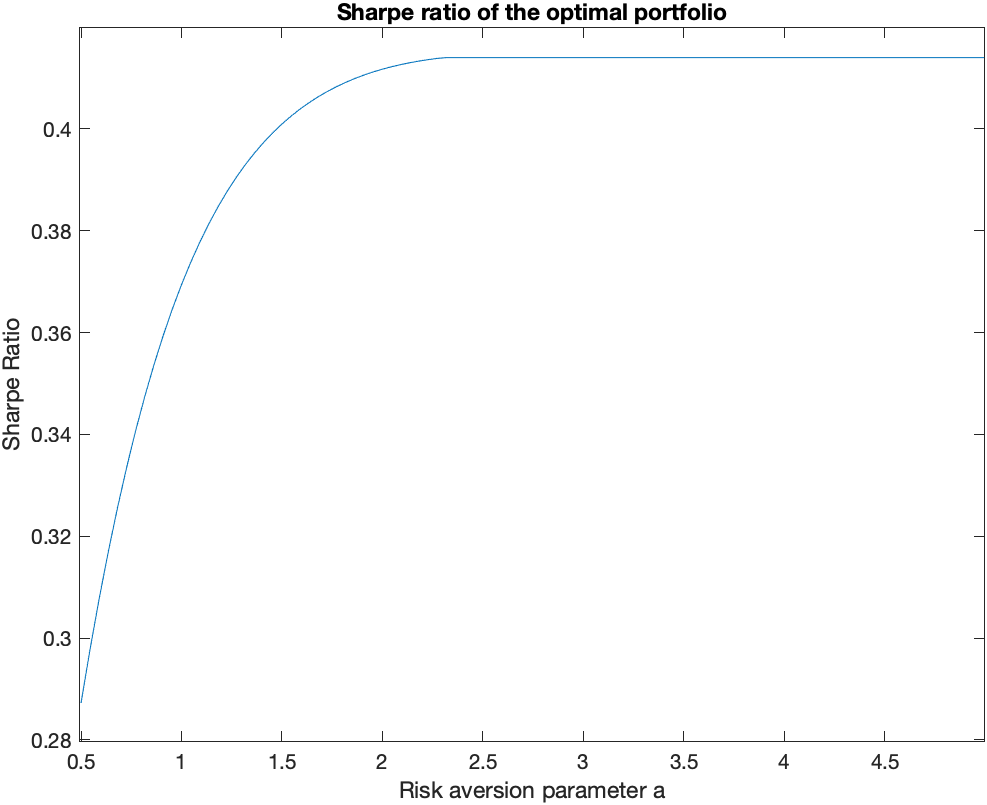
\includegraphics[scale = 0.8]{Figures/SharpeRatio.png}
    \caption{Sharpe Ratios in function of the risk aversion}
    \label{SR}
  \end{figure}
  
  
  \end{itemize}

\end{exercise}

\newpage

\begin{exercise}{2}

	(a) We recall the equation for computing the excess returns considering the one factor regression:
	
	\begin{align*}
		R_{i}^{e} = \alpha_{i} + \beta_{i}R_{M}^{e}  + \epsilon_{i} \forall i
	\end{align*}
	
	The expected profit (in dollars) is therefore:
	
	\begin{align*}
		1'000'000 \times (0.01 + 1 \times R_{M}^{e}) - 1'000'000 \times (	-0.01 + 1 \times R_{M}^{e}) = 20'000 \$
	\end{align*}		

	The standard deviation is computed as follows:
	
	\begin{align*}
		\sqrt{10 \times \left( \frac{2'000'000}{10} \times 0.20 \right)^{2}} = 126'491.11 
	\end{align*}

	(b) For 40 or 100 stocks, the expected profit will not change since there are as many stocks with positive alpha that there are with negative alpha.
	
	\smallbreak
	
	The standard deviation however will change. For 40 stocks:
	
	\begin{align*}
		\sqrt{40 \times \left( \frac{2'000'000}{40} \times 0.20 \right)^{2}} = 63'245.55
	\end{align*}
	
	For 100 stocks:
	
	\begin{align*}
		\sqrt{100 \times \left( \frac{2'000'000}{100} \times 0.20 \right)^{2}} = 40'000.00
	\end{align*}

	As the number of stocks increases, the volatility decreases.

\end{exercise}

\newpage

\begin{exercise}{3}

	(b) After downloading the data, we compute the annualized mean, standard deviation, and sharpe ratio of BRK excess returns, the three Fama-French factors ($R_{m}^{e}$, $SMB$, $HML$), the momentum ($MOM$), and the risk free rate:

	\begin{table}[h!]
		\centering
 		\begin{tabular}{||c c||} 
 			\hline
 			& Annualized mean \\ [0.5ex] 
 			\hline\hline
 			BRK excess returns & 0.185343 \\ 
 			$R_{m}^{e}$ & 0.078565 \\
 			SMB & 0.024547 \\
 			HML & 0.027563 \\
 		    MOM & 0.075058 \\
 			Risk-free & 0.043717 \\ [1ex] 
 			\hline
		 \end{tabular}
	\end{table}	

	\begin{table}[h!]
		\centering
 		\begin{tabular}{||c c||} 
 			\hline
 			& Annualized standard deviation \\ [0.5ex] 
 			\hline\hline
 			BRK excess returns & 0.231796 \\ 
 			$R_{m}^{e}$ & 0.151624 \\
 			SMB & 0.099633 \\
 			HML & 0.099377 \\
 		    MOM & 0.151413 \\
 			Risk-free & 0.010153 \\ [1ex] 
 			\hline
		 \end{tabular}
	\end{table}	

	\begin{table}[h!]
		\centering
 		\begin{tabular}{||c c||} 
 			\hline
 			& Annualized sharpe ratio \\ [0.5ex] 
 			\hline\hline
 			BRK excess returns & 0.610997 \\ 
 			$R_{m}^{e}$ & 0.229836 \\
 			SMB & -0.192405 \\
 			HML & -0.162549 \\
 		    MOM & 0.206992 \\
 			Risk-free & 0.0 \\ [1ex] 
 			\hline
		 \end{tabular}
	\end{table}	
	
	(c) We then run various regressions, where we report the estimated $\alpha$, $\beta s$ along with the associated $t$-statistics, $R^{2}$, and information ratio of BRK. We proceed with the first regression
	
	\begin{align*}
		R_{t}^{e} = \alpha + \beta_{1}R^{e}_{mt} + \epsilon_{t} 
	\end{align*}
	
	\begin{table}[h!]
		\centering
 		\begin{tabular}{||c c c c c||} 
 			\hline
 			Regression 1 & Full-sample data & $t$ & Data until 1995 & \\ [0.5ex] 
 			\hline\hline
 		  	& Value & $t$-stat & Value & $t$-stat\\ [0.5ex] 
 			\hline\hline
 			$\alpha$ & 0.011 & 4.121 &  0.019 & 4.204\\ 
 			$\beta_{1}$ & 0.684 & 11.363 & 0.898 & 8.696\\ [1ex]
 			\hline\hline
 			$R^{2}$ & 0.200 & & 0.249 &\\
 			IR & 0.635 & & 0.975 &\\ [1ex] 
 			\hline
		 \end{tabular}
	\end{table}	

	The second regression
	
	\begin{align*}
		R_{t}^{e} = \alpha + \beta_{1}R^{e}_{mt} + \beta_{2}SMB_{t}+ \beta_{3}HML_{t} + \epsilon_{t} 
	\end{align*}
	
	\begin{table}[h!]
		\centering
 		\begin{tabular}{||c c c c c||} 
 			\hline
 			Regression 2 & Full-sample data &  & Data until 1995 & \\ [0.5ex] 
 			\hline\hline
 		  	& Value & $t$-stat & Value & $t$-stat\\ [0.5ex]  
 			\hline\hline
 			$\alpha$ & 0.009 & 3.659 & 0.016 & 3.460\\ 
 			$\beta_{1}$ & 0.810 & 13.115 & 0.996 & 8.399\\
 			$\beta_{2}$ &  -0.245 & -2.683 & 0.225 & 1.213\\
 			$\beta_{3}$ & 0.502 & 5.443 & 0.475 & 2.349\\ [1ex]
 			\hline\hline
 			$R^{2}$ & 0.256 & & 0.271 &\\
 			IR & 0.570 & &  0.833 &\\ [1ex] 
 			\hline
		 \end{tabular}
	\end{table}

	The third regression
	
	\begin{align*}
		R_{t}^{e} = \alpha + \beta_{1}R^{e}_{mt} + \beta_{2}SMB_{t}+ \beta_{3}HML_{t} + \beta_{4}MOM_{t} \epsilon_{t} 
	\end{align*}

	\begin{table}[h!]
		\centering
 		\begin{tabular}{||c c c c c||} 
 			\hline
 			Regression 3 & Full-sample data & & Data until 1995 & \\ [0.5ex] 
 			\hline\hline
 		  	& Value & $t$-stat & Value & $t$-stat\\ [0.5ex] 
 			\hline\hline
 			$\alpha$ & 0.009 & 3.375 &  0.016 & 3.218\\ 
 			$\beta_{1}$ & 0.823 & 13.087 & 0.991 & 8.267\\
 			$\beta_{2}$ &  -0.250 & -2.740 & 0.223 & 1.203\\
 			$\beta_{3}$ &  0.531 & 5.546 & 0.486 & 2.368\\
 			$\beta_{4}$ & 0.068 & 1.121 & 0.049 & 0.336\\ [1ex]
 			\hline\hline
 			$R^{2}$ & 0.258 & & 0.271 &\\
 			IR & 0.537 & &  0.810 &\\ [1ex] 
 			\hline
		 \end{tabular}
	\end{table}
	
	The last regression
	
		\begin{align*}
		R_{t}^{e} = \alpha + \beta_{1}R^{e}_{mt} + \beta_{2}SMB_{t}+ \beta_{3}HML_{t} + \beta_{4}MOM_{t} + \beta_{5}RMW_{t} + \beta_{6}CMA_{t} + \epsilon_{t} 
	\end{align*}

	\begin{table}[h!]
		\centering
 		\begin{tabular}{||c c c c c||} 
 			\hline
 			Regression 4 & Full-sample data & & Data until 1995 & \\ [0.5ex] 
 			\hline\hline
 		  	& Value & $t$-stat & Value & $t$-stat\\ [0.5ex] 
 			\hline\hline
 			$\alpha$ & 0.007 & 3.375 & 0.013 &  2.580\\ 
 			$\beta_{1}$ & 0.857 & 13.018 & 1.011 & 8.214\\
 			$\beta_{2}$ &  -0.126 & -1.300 & 0.289 & 1.485\\
 			$\beta_{3}$ &  0.478 & 3.666 & 0.572 & 1.858\\
 			$\beta_{4}$ &  0.037 & 0.602 & 0.018 & 0.118\\
 			$\beta_{5}$ &  0.436 & 3.434 & 0.450 & 1.142\\
 			$\beta_{6}$ & 0.001 & 0.006 & 0.099 & 0.220\\ [1ex]
 			\hline\hline
 			$R^{2}$ & 0.275 & & 0.275 &\\
 			IR & 0.443 & & 0.702 &\\ [1ex] 
 			\hline
		 \end{tabular}
	\end{table}

  (d) The RMW (Robust-minus-Weak) and the CMA (Conservative-minus-Aggresive)
  factors are constructed in a fashion similar to the HML where instead of the
  book-to-market ratio, the stocks are sorted by the \textit{OP} (\text{operating
    profitability}) and \textit{Inv} (expected growth of book equity, i.e.
  investment). The RMW and the CMA are then the differences between the returns
  of two portfolios - one formed of some top quintile and second of a bottom
  quintile in the underlying metric. Fama and French argue that these two
  factors are a meaningful addition to the model as a replacement of the
  book-to-market ratio. Indeed, nowadays, several tech firms seem to reap
  returns by unstinting investment in spite of null operational profitability
  (ex. Amazon). Why SML can be dropped if RMW and CMA are introduced? It goes
  back to the Miller-Modigliani theory of the market value of a firm's stock as
  the discounted sum of its future earnings minus investments:

  \begin{equation}
    \frac{M_t}{B_t} = \frac{\sum_{\tau = 1}^\infty(Y_{t + \tau} - d B_{t + \tau})/(1 + r)^\tau}{B_t}
  \end{equation}
where $Y_{t + \tau}$ is total equity earnings for period $t + \tau$, $dB_{t
  + \tau}$ is the change in total book equity, $r$ is the expected stock return
and $M_t$ and $B_t$ are the market and the book value of the firm at time $t$.
One observes that for a fixed book-to-market ratio $B_t / M_t$, the expected
stock return $r$ can be written as a function of the expected earnings
(operational profitability) and as
a function of the firms book equity (investments). Controlling on these two
factors would render the book-to-market ratio redundant. 

(e)

An interpretation of the betas in the Regression 4 can help us assess what kind
of investor Warren Buffet is. First of all, (1) his firm has less market exposure
than the market portfolio ($\beta_1 < 1$). This holds true even in the current
crisis of indiscriminate stock sell off caused by the coronavirus: while the S\&P 500 dropped $29\%$
from March 2 to March 23, the BRK stock price dropped by $27 \%$ in the same
time period. Warren Buffet
is a (2) value investor. The Berkshire Hathaway has a negative exposure to the
SMB factor which means that when the small stocks outperform big stocks, Buffet
takes a hit. A personal quote of Buffet catches him saying that 'Life is like a
snowball. The important thing is finding wet snow and a really long hill.' His
personal philosophy translates directly into his investment strategy: Buffet
makes few, but important investment decisions. This makes him miss-out on the
precipitous growth of certain small stocks, information which investors factoring in by lowering the price of his
shares in such instances. Positive factor loadings of $\beta_3 = 0.478$ and $\beta_5 = 0.436$ for
High-minus-Low book-to-market ratios and Robust-minus-Weak factors show that
Buffet invests in firms with strong fundamentals that demonstrate potential
for persistent profitability. On the other hand, low MOM and CMA loadings corroborate
that Buffet is (4) not driven by Market momentum and does not discriminate
between firms with aggressive or conservative investments policies, as long as
they can sustain their profits.

(f) From the simple Regression 1 which controls only for systematic risk to
Regression 4 which controls for a variety of factors, the alpha of Warren Buffet
decreases from $\alpha_1 = 1.1\%$ to $\alpha_4 = 0.7 \%$ which is not dramatic
considering the multitude of controlling factors in Regression 4. The
information ratio IR decreases from $IR_1 = 0.635$ to $IR_4 = 0.443$. Therefore, the
exposure to common risk factors is far from explaining the full genius of Warren
Buffet. It would have explained the outperformance of Buffett only if the
$\alpha_4$ would have been close to 0.


(g) In order to construct a maximum Sharpe Ratio portfolio (which is a mean-variance
optimal portfolio) out of the 6 factor portfolios $R^e_M$, $SMB$, $HML$, $MOM$,
$RMW$, $RMW$, $CMA$, the Berkshire Hathaway and the riskless T-bill, we have to
determine the $IR$ of each of the securities and their corresponding $\alpha$'s
and $\sigma$'s. The Sharpe Ratio of the efficient portfolio will then be

\begin{equation}
  SR_P = \sqrt{SR_F^2 + \sum_{i = 1}^n IR^2_i}
\end{equation}

We compute the needed statistics such as $IR^2$, $\alpha$ and $\sigma$ by
regressing each factor on all the previous factors in the ordered list. This
makes sure that the $\epsilon_i$ are indeed uncorrelated. Then, we invest $x_i =
\frac{\alpha_i}{a \sigma_i^2}$ in each portfolio with an $a = \frac{SR_P}{0.20}
\approx 6.840$ corresponding to our risk preference of $20\%$ of volatility. In the table
below, we summarize these statistics:

\begin{table}[h!]
  \centering
  \begin{tabular}{||c c c c c||} 
    \hline
    Factor & $\alpha_i$ & $\sigma_i$ & $IR_i$ &  $x_i$ \\
    \hline\hline
    $R_f$ & - & - & 0 &  -5.733 \\
    $R_M$ & 0 & 0.043 & $SR_F = $ 0.518 & 1.734 \\
    $SMB$ & 0.001 & 0.028 & 0.130 &  0.197 \\
    $HML$ & 0.004 & 0.028 & 0.442 & 0.677 \\
    $MOM$ & 0.008 & 0.042 & 0.694 & 0.703 \\
    $RMW$ & 0.004 & 0.020 & 0.652 & 1.380 \\
    $CMA$ & 0.002 & 0.013 & 0.535 & 1.715 \\
    $BRK$ & 0.007 & 0.057 & 0.443 & 0.328 \\
    \hline\hline
    \end{tabular}
    \caption{Period 1976 - 2019}
\end{table}

As it is seen in the table above, the resulting portfolio is highly leveraged,
with considerable weights corresponding to the market portfolio,
Robust-minus-Weak portfolio and
Conservative-minus-aggressive investment portfolio. The Berkshire Hathaway
investment represents only $0.328/6.733 \approx 4,87 \%$ of the total investment
in stocks. This is convincing since Berkshire Hathaway has a lot of firm-specific risk
which needs to be diluted for the portfolio to by well-diversified and efficient.

	
	(h) We process similarly as in part (c) but this time with data until 1995.
  See tables in part (c). 

  Put side by side, the regression results on the full-sample data and data
  until 1995, call to mind the stark contrast in the performance of the firm. It
  seems that till 1995, the firm has outperformed itself by a factor of two
  times, when compared to itself during the period from 1976 to 2019.
  Moreover, the exposure to Small-minus-Big stocks has been higher, even
  positive, for the data until 1995. The exposure to the market  has been 
  higher (close to $\beta_1 = 1$) as well. To explain these results, we have to consider
  what Berkshire Hathaway does to make profit. Tersely put, it invests in firms
  by buying them, i.e. Buffet acquires and merges firms. Over time, the acquired
  firms grow in value and the profits allow for more expensive deals. For
  example, from the publicly available data, most of the acquisitions before
  1995 were priced below \$1 billion while in 1995, a big acquisition of General
  Reinsurance Corporation for \$ 22 billion and the ensuing bigger firms have
  tilted Buffett's portfolio towards big stocks.
  
  With a larger portfolio of acquired assets, it is expected that consistently maintaining
   a positive $\alpha$ is less feasible. This is corroborated by
  theory we have covered in class: in large portfolios (such as Buffett's nowadays),
  most assets have to have close to zero alphas. Buffett has also published a
  number of books revealing his investing genius. It is a safe assumption to
  say that his popularity has only amplified his reach and impact on the
  investment craft. As such, many have learned some of his secrets of investment
  and management which presumably allowed them to reach for those positive
  alphas for themselves, canceling out Buffett's uncommon big alpha.

\end{exercise}
  
\end{document}
